\documentclass[11pt]{article}

\usepackage[review]{acl}
\usepackage{times}
\usepackage{latexsym}
\usepackage[T1]{fontenc}
\usepackage[utf8]{inputenc}
\usepackage{booktabs}
\usepackage{amsmath}
\usepackage{amssymb}
\usepackage{graphicx}
\usepackage{tikz}
\usepackage{multirow}
\usepackage{enumitem}
\usepackage{xcolor}
\usepackage{subcaption}
\usetikzlibrary{arrows.meta, positioning, calc, fit, backgrounds}

\newcommand{\ph}[1]{\textcolor{red!70!black}{#1}}

\title{Ontology-Driven Clustering for Extracting Legal Reasoning Graphs}

\author{Anonymous}

\begin{document}
\maketitle

\begin{abstract}
Extracting structured reasoning from long court judgments is a persistent challenge in legal NLP: large language models can identify individual legal concepts but struggle to consistently link them across thousands of tokens, producing graphs that are incomplete, structurally invalid, or non-reproducible. We present \textsc{LexCGraph}, a pipeline that decomposes long-document graph extraction into a set of local inference problems by clustering extracted nodes around canonical legal concepts defined in a compiled ontology. Within each cluster, an LLM infers edges under ontology-provided constraints (definitions, AND/OR requirements, defeaters, relation whitelists); all cross-cluster structure is constructed deterministically. On 2,517 Indian Supreme Court cases from IL-TUR, ontology-normalized annotations outperform BM25 by +0.100 nDCG@10 ($p < 0.05$) and all dense retrieval baselines. Graph representations improve zero-shot outcome prediction by +11.1pp on Grok-4.1 and +11.1pp on Claude Sonnet 4.5 (McNemar $p < 0.05$), with substantially improved calibration (ECE: 0.109$\rightarrow$0.026). Crucially, structured nodes \emph{without} ontology-constrained edges perform \emph{worse} than raw text, demonstrating that naive structuring destroys implicit textual signals---only ontology-constrained relational structure recovers and exceeds them. A leakage audit confirms comparable information access between representations (0.233 vs.\ 0.225 signals per 1K characters), and the consistent performance ordering across representations rules out LLM memorization. An ontology completeness ablation (11 vs.\ 54 concepts) reveals that enrichment dramatically improves graph quality (gold tier: 77\%$\rightarrow$90\%, pseudo-cluster nodes: 93\% reduction) while prediction accuracy remains unchanged---indicating that core doctrines saturate outcome-predictive signal while additional concepts improve structural fidelity for downstream applications. The AND/OR justification structure enables counterfactual impact analysis: across 15,276 justification sets, 77.5\% of holdings are structurally fragile, and removing the single most critical concept eliminates one-third of a case's justifications on average. \ph{Cross-jurisdictional evaluation on ECHR cases confirms generalizability.} We release the ontology, extraction code, and evaluation scripts.\footnote{Code: \url{https://anonymous.4open.science/r/lexcgraph}}
\end{abstract}

\begin{figure*}[t]
  \centering
  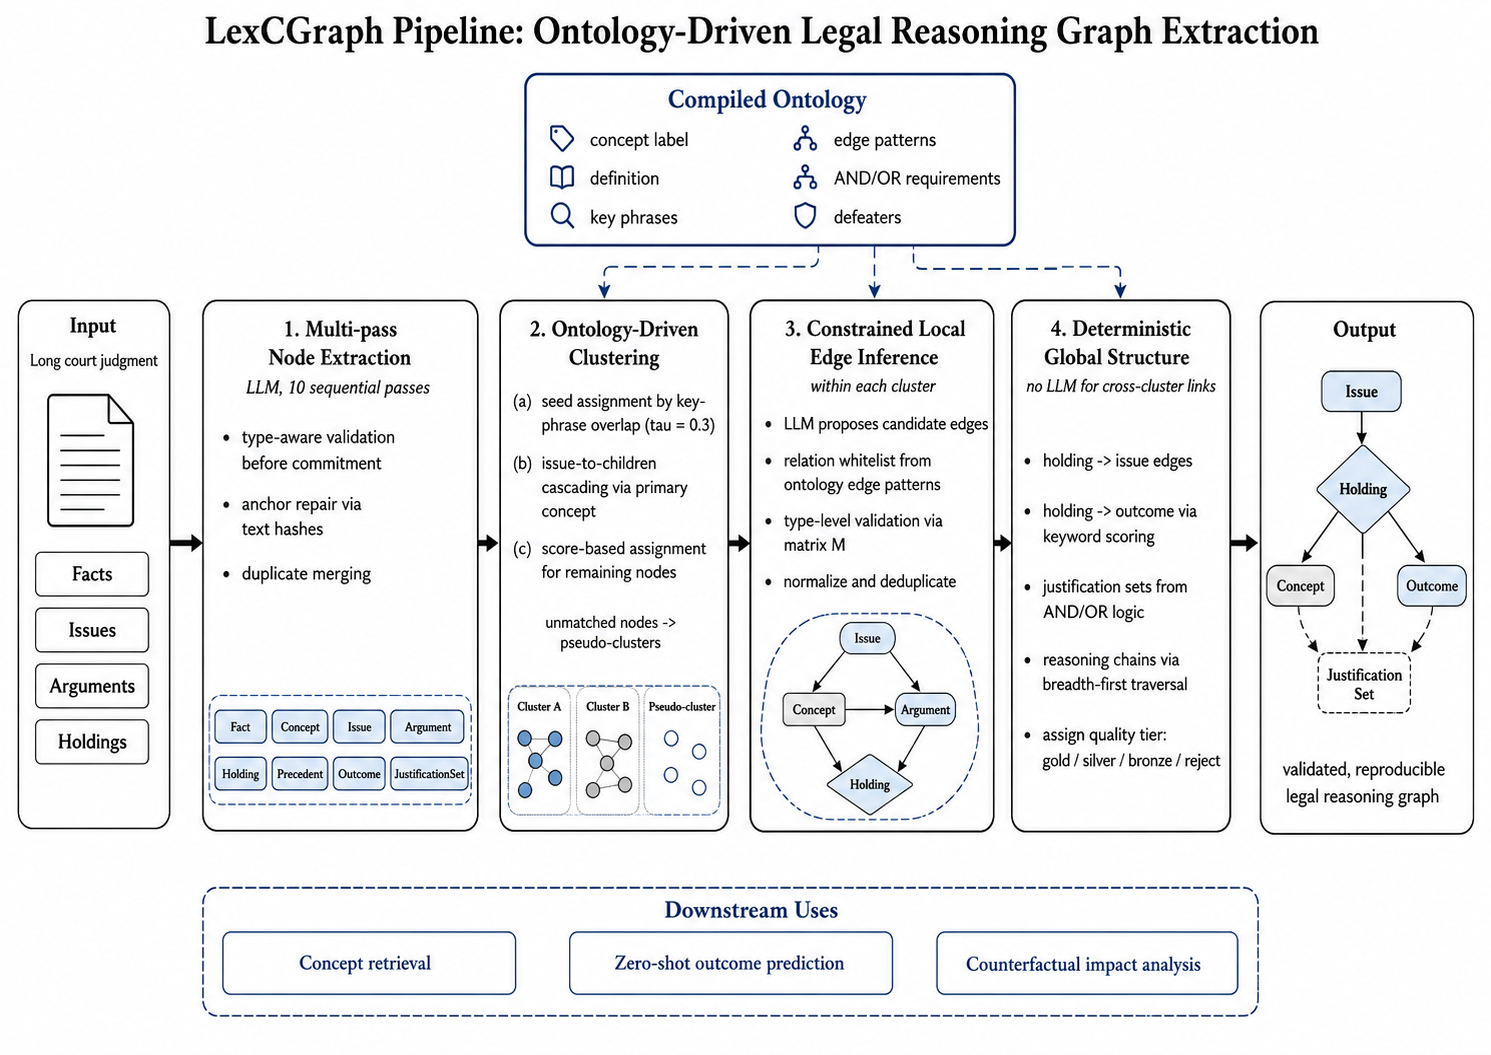
\includegraphics[width=\textwidth]{pipeline.png}
  \caption{Overview of the \textsc{LexCGraph} pipeline. A compiled ontology provides concept definitions, key phrases, edge patterns, AND/OR requirements, and defeaters. The four-stage pipeline decomposes long-document graph extraction into local inference problems, producing validated legal reasoning graphs for concept retrieval, zero-shot outcome prediction, and counterfactual impact analysis.}
  \label{fig:pipeline}
\end{figure*}

% ============================================================
\section{Introduction}
% ============================================================

Court judgments are long, multi-issue documents whose reasoning is distributed across factual findings, statutory interpretation, doctrine-specific tests, and citations to precedent. Capturing this reasoning in structured form is essential for legal case retrieval, explainability, and corpus-level legal analytics---yet the very properties that make court reasoning rich also make it difficult to extract: legally relevant spans are separated by thousands of tokens, doctrinal tests involve conjunctive and disjunctive requirements that must be tracked jointly, and the same abstract legal concept manifests differently across jurisdictions.

Large language models can extract individual nuggets of information from legal text, but they struggle to consistently link distant items across long inputs. When tasked with end-to-end graph extraction from a 15,000-token judgment, LLMs frequently produce graphs that are incomplete, structurally invalid, or non-reproducible. These failures are not primarily linguistic---the models understand the text---but combinatorial: the space of possible edges grows quadratically with the number of extracted nodes, and without structural constraints, the model must navigate this space with only implicit knowledge of legal reasoning patterns.

We propose \textsc{LexCGraph}, an ontology-driven approach that addresses this problem by decomposing long-document graph extraction into a set of \emph{local} inference problems. The key mechanism is \textbf{ontology-driven clustering}: extracted nodes are assigned to clusters defined by canonical legal concepts in a compiled ontology, and edge inference is restricted to within-cluster pairs using ontology-provided constraints. All cross-cluster structure is constructed deterministically. This design yields three properties: (1)~\emph{reproducibility}---the same input always produces the same graph; (2)~\emph{structural validity}---every edge satisfies type-level constraints; and (3)~\emph{counterfactual traceability}---the AND/OR justification structure enables deterministic impact analysis when a concept node is removed.

Our evaluation reveals several findings with implications beyond legal NLP. First, ontology-constrained graphs substantially outperform raw text on zero-shot prediction (+11.1pp) and concept retrieval (+0.100 nDCG@10). Second, and more surprisingly, structured nodes \emph{without} ontology-constrained edges perform \emph{worse} than raw text---demonstrating that naive structuring destroys implicit textual signals (discourse cues, paragraph structure, narrative flow) without replacing them with relational structure. Third, an ontology completeness ablation shows that expanding from 11 to 54 concepts dramatically improves graph structural quality (gold tier: 77\%$\rightarrow$90\%) without changing prediction accuracy, indicating that core doctrinal concepts saturate outcome-predictive signal. Fourth, a facts-only experiment confirms that the pipeline's value derives from structuring \emph{judicial reasoning}---the analytical connections between doctrines, precedents, and holdings---not from reorganizing factual content: graphs extracted from case facts alone provide no prediction advantage. These findings collectively establish that the graph's value lies in structured representation of reasoning, not in information advantage or superficial reorganization.

\paragraph{Contributions.}
\begin{enumerate}[nosep,leftmargin=*]
\item \textbf{Ontology-driven clustering for legal graph extraction}: a method that decomposes long-document graph construction into local inference problems scoped by ontology-defined concept clusters, producing reproducible, structurally validated graphs with deterministic cross-cluster structure (\S\ref{sec:method}).
\item \textbf{Multi-dimensional evaluation}: prediction, retrieval, calibration, ontology completeness ablation, facts-only control, leakage audit, and counterfactual structural analysis---establishing both the value and the boundaries of graph-based legal reasoning (\S\ref{sec:results}).
\item \textbf{Counterfactual impact analysis}: a domain-grounded explainability mechanism enabled by AND/OR justification logic, with corpus-level structural statistics across 15,276 justification sets (\S\ref{sec:counterfactual}).
\item \textbf{Resources}: a compiled legal ontology (54 fully-specified concepts), extraction code, and evaluation scripts.
\end{enumerate}

% ============================================================
\section{Related Work}
\label{sec:related}
% ============================================================

\paragraph{Legal NLP and judgment prediction.}
LexGLUE \cite{chalkidis2022lexglue} and LegalBench \cite{guha2023legalbench} standardize legal NLP evaluation; IL-TUR extends evaluation to Indian law with the CJPE task \cite{joshi2024iltur}, derived from ILDC \cite{malik2021ildc}. For ECHR prediction, \citet{chalkidis2019neural} established neural baselines; COLIEE \cite{rabelo2022coliee} benchmarks statute retrieval. Structured prediction approaches model subtask dependencies as DAGs \cite{zhong2018topological}, apply relational learning \cite{dong2021relational}, and survey the state of the art \cite{feng2022survey}. Our work differs in extracting the reasoning structure itself as a first-class output, rather than using implicit structure to improve a classifier.

\paragraph{Legal knowledge graphs and ontologies.}
The LKIF Core ontology \cite{hoekstra2007lkif} provides foundational concepts for legal knowledge interchange; \citet{kucuk2025computational} survey datasets, benchmarks, and ontologies for computational law. \citet{sarika2022kg} build a knowledge graph from Indian judgments using rule-based NER; \citet{dhani2024similar} combine legal KGs with GNNs for case similarity. Our approach uses the ontology not merely as a schema but as a \emph{constraint} on the extraction process---scoping which edges the LLM may propose and enforcing structural validity at each step.

\paragraph{Structure-aware legal retrieval.}
\citet{li2023sailer} pre-train a structure-aware model for legal case retrieval, \citet{ma2023structural} show structural information improves retrieval, and \citet{tang2024caselink} use inductive graph learning. \citet{trippas2025reproducibility} study reproducibility of graph-based retrieval---a problem our deterministic cross-cluster structure directly addresses.

\paragraph{Argumentation mining and graph reasoning.}
\citet{toulmin1958uses} provides the foundational claim/grounds/warrant abstraction; \citet{mochales2011argumentation} and \citet{wyner2010approaches} developed automatic argumentation extraction from legal texts. Graph-of-Thoughts \cite{besta2024got} models LLM reasoning as graph traversal but enforces no domain-specific constraints. Unlike graph counterfactual explainers that perturb edges to flip black-box predictions \cite{tan2022counterfactual}, our AND/OR justification structure enables domain-grounded counterfactual analysis that mirrors legal reasoning practice (\S\ref{sec:counterfactual}).

% ============================================================
\section{Method}
\label{sec:method}
% ============================================================

\textsc{LexCGraph} extracts a legal reasoning graph from a court decision in four stages: (1)~multi-pass node extraction, (2)~ontology-driven clustering, (3)~constrained local edge inference, and (4)~deterministic global structure construction.

\subsection{Graph Schema}
\label{sec:schema}

Each decision is represented as a typed, anchored graph $G = (V, E, A)$. The schema defines eight node types (Fact, Concept, Issue, Argument, Holding, Precedent, Outcome, JustificationSet) and 32 edge relations derived from ontology edge patterns and legal argumentation literature \cite{toulmin1958uses,mochales2011argumentation}. A type-level validation matrix $M \in \{0,1\}^{|T| \times |T| \times |R|}$ specifies permitted relations between each pair of node types. Edges are normalized through an alias mapping layer (${\sim}200$ aliases $\rightarrow$ 32 canonical relations) and deterministically deduplicated.

\subsection{Compiled Ontology}
\label{sec:ontology}

The compiled ontology serves dual roles: defining cluster keys and providing extraction constraints. Each concept includes: (1)~label and definition, (2)~key phrases for node-to-cluster assignment, (3)~typical edge patterns constraining intra-cluster inference, (4)~AND/OR requirements encoding conjunctive/disjunctive test structures, and (5)~defeaters specifying blocking conditions.

The Indian ontology contains 54 fully-specified concepts: 11 constitutional doctrines (e.g., Basic Structure, Maneka Gandhi proportionality framework, Wednesbury Unreasonableness) with complete AND/OR reasoning structures, and 43 offense, procedural, and evidence concepts (e.g., Murder, Regular Bail, Electronic Evidence, Dying Declaration) with legal elements, defenses, establishing cases, and key phrases. All concepts were verified against primary legal sources with landmark case citations validated by independent audit (\S\ref{sec:limitations}). Appendix~\ref{app:ontology} provides representative examples spanning each concept category and jurisdiction.

\paragraph{Concrete example: proportionality.}
The Maneka Gandhi proportionality framework is encoded as a six-part AND test: procedure by law must exist; it must be ``right, just and fair''; not ``arbitrary, fanciful or oppressive''; must satisfy Article~14 (non-arbitrariness); Article~19 (reasonableness); and conform to natural justice. Defeaters include express statutory exclusion and emergency situations. Key phrases include ``just, fair and reasonable'' and ``Golden Triangle.'' This structure scopes LLM edge inference: within a proportionality cluster, the LLM may only propose edges from the concept's relation whitelist, and each proposed edge is validated against the type-level matrix $M$.

\subsection{Extraction Pipeline}
\label{sec:pipeline}

\paragraph{Stage 1: Multi-pass node extraction.}
Ten sequential passes with Grok-4.1, each validated before commitment: the type-aware matrix rejects invalid node types, anchors are repaired via text hashes, and duplicates are merged.

\paragraph{Stage 2: Ontology-driven clustering.}
Nodes are assigned to concept clusters via three phases: (1)~seed assignment from key-phrase overlap ($\tau = 0.3$), (2)~cascading of Issue nodes to children via primary-concept fields, and (3)~score-based assignment for remaining nodes. Unmatched nodes enter pseudo-clusters with conservative constraints. Each cluster is summarized into a structured context record containing concept definition, AND/OR requirements, defeaters, and candidate node mentions.

\paragraph{Stage 3: Constrained local edge inference.}
Within each cluster, an LLM proposes edges under two constraints: a relation whitelist from the ontology's edge patterns, and type-level validation via matrix $M$. Proposed edges are normalized and deduplicated.

\paragraph{Stage 4: Deterministic global structure.}
All cross-cluster structure is constructed without LLM involvement: \texttt{resolves} edges from holdings to issues, \texttt{determines} edges from holdings to outcomes via keyword scoring, justification sets compiling intra-cluster evidence under AND/OR logic, and reasoning chains via breadth-first traversal. Each graph receives a quality tier (gold/silver/bronze/reject).

% ============================================================
\section{Experimental Setup}
\label{sec:setup}
% ============================================================

\subsection{Dataset and Task}

We evaluate on 2,517 IL-TUR CJPE cases \cite{joshi2024iltur} (838 accepted, 1,679 rejected; stratified, seed=42). For zero-shot outcome prediction, we compare two input representations, both identically blinded: (i)~\textit{Raw}: decision text with outcome-revealing content removed via regex filtering; and (ii)~\textit{Graph}: linearized reasoning graph with outcome-bearing fields withheld.

\subsection{Models and Metrics}

We evaluate on two architecturally distinct frontier models: Grok-4.1 and Claude Sonnet 4.5. Since Grok also serves as the extraction model, Sonnet provides an independent cross-model control. We measure accuracy, macro-F1, calibration (ECE, Brier), and use McNemar's test with bootstrap 95\% CIs. For retrieval, we report nDCG@10, MAP, and P@10 with paired $t$-tests. Our evaluation across 10,068 model runs produced zero parse or API errors.

% ============================================================
\section{Results}
\label{sec:results}
% ============================================================

\subsection{Outcome Prediction}

\begin{table}[t]
\small
\centering
\caption{Zero-shot CJPE outcome prediction on 2,517 IL-TUR cases. Graph inputs outperform raw text on both models across all metrics.}
\label{tab:main_results}
\begin{tabular}{llcccc}
\toprule
Model & Input & Acc. & F1 & ECE$\downarrow$ & Brier$\downarrow$ \\
\midrule
\multirow{2}{*}{Grok-4.1} & Raw & .742 & .722 & .109 & .195 \\
 & Graph & \textbf{.853} & \textbf{.839} & \textbf{.026} & \textbf{.120} \\
\midrule
\multirow{2}{*}{Sonnet 4.5} & Raw & .663 & .631 & .091 & .228 \\
 & Graph & \textbf{.774} & \textbf{.754} & \textbf{.010} & \textbf{.174} \\
\bottomrule
\end{tabular}
\end{table}

Table~\ref{tab:main_results} shows that graphs consistently outperform raw text. Accuracy improves by +11.1pp on Grok and +11.1pp on Sonnet (McNemar $\chi^2$=119.97 and 92.34; $p < 0.05$), with bootstrap 95\% CIs excluding zero. Calibration improves markedly: ECE drops from 0.109$\rightarrow$0.026 on Grok, with raw text systematically overconfident in the 0.70--0.90 range while graph inputs track the reliability diagonal closely.

\subsection{Structure vs.\ Structured Nodes}

\begin{table}[t]
\small
\centering
\caption{Ablation: Full Graph vs.\ Structured Nodes (same nodes, no edges) vs.\ Raw text. Structured nodes without edges perform \emph{worse} than raw text. $\dagger$McNemar $p < 0.05$.}
\label{tab:ablation}
\begin{tabular}{llccc}
\toprule
Model & Metric & Full Graph & Struct.\ Nodes & Raw \\
\midrule
\multirow{2}{*}{Grok-4.1} & Acc. & \textbf{0.864}$^\dagger$ & 0.718 & 0.739 \\
 & Brier$\downarrow$ & \textbf{0.113} & 0.211 & 0.196 \\
\midrule
\multirow{2}{*}{Sonnet 4.5} & Acc. & \textbf{0.771}$^\dagger$ & 0.683 & 0.663 \\
 & Brier$\downarrow$ & \textbf{0.175} & 0.219 & 0.228 \\
\bottomrule
\end{tabular}
\end{table}

Table~\ref{tab:ablation} reveals a striking finding: structured nodes without ontology-constrained edges perform \emph{worse} than raw text on both models. On Grok, structured nodes achieve 0.718 accuracy versus 0.739 for raw text. This demonstrates that merely extracting and labeling legal concepts can \emph{destroy} implicit textual signals---discourse cues, paragraph structure, narrative flow---without replacing them with relational structure. Only when ontology-constrained edges, justification sets, and reasoning chains are added does the graph representation substantially exceed both baselines. The consistent performance ordering across representations (full graph $>$ raw text $>$ structured nodes) using identical models and cases rules out LLM memorization as an explanation: if models recognized cases from pretraining, performance would be independent of input representation.

\subsection{Ontology Completeness Ablation}

\begin{table}[t]
\small
\centering
\caption{Ontology completeness ablation. Expanding from 11 to 54 concepts dramatically improves graph quality while prediction accuracy remains unchanged.}
\label{tab:ont_ablation}
\begin{tabular}{lcc}
\toprule
Metric & 11 concepts & 54 concepts \\
\midrule
Prediction accuracy & 0.855 & 0.853 \\
Gold tier graphs & 77.1\% & 90.3\% \\
UNLISTED nodes/graph & 47.4 & 3.2 \\
Edges/graph & 108.8 & 116.0 \\
Unique concept IDs & 14,064 & 1,634 \\
\bottomrule
\end{tabular}
\end{table}

To assess the marginal value of ontology investment, we expanded the Indian ontology from 11 fully-specified doctrinal concepts to 54 concepts (adding 43 offense, procedural, and evidence concepts with complete legal elements, defenses, and key phrases) and re-ran the full pipeline on the same 2,517 cases.

Table~\ref{tab:ont_ablation} reveals a dissociation between graph quality and prediction accuracy. Graph structural quality improved dramatically: gold-tier graphs increased from 77.1\% to 90.3\%, pseudo-cluster (UNLISTED) node assignments dropped by 93\% (47.4$\rightarrow$3.2 per graph), and 14,064 ad-hoc pseudo-concept IDs collapsed into 1,634 canonical ontology concepts. However, prediction accuracy was statistically unchanged (0.855 vs.\ 0.853, $p > 0.05$).

This indicates that the 11 core doctrinal concepts---proportionality, natural justice, reasonable classification, Wednesbury unreasonableness, and others---capture the reasoning structure predictive of case outcomes. The additional 43 offense-level and procedural concepts improve structural completeness for applications requiring fine-grained graph fidelity (retrieval, explainability, counterfactual analysis) without contributing additional predictive signal for binary outcomes.

\subsection{Facts-Only Control}

A natural question is whether the pipeline's value derives from structuring judicial reasoning or merely from reorganizing factual content. To test this, we extracted graphs from only the facts section of 50 cases (the same input available to supervised ILDC baselines) and compared prediction accuracy across three conditions: raw facts (64\%), facts-only graph (62\%), and full graph (90\%). The facts-only graph provides no prediction advantage, confirming that the pipeline's value derives from structuring the court's analytical reasoning---the connections between doctrines, precedents, and holdings---not from reorganizing facts. This situates \textsc{LexCGraph} as a reasoning structure extraction tool rather than a fact enhancement method.

\subsection{Fairness Controls}

\paragraph{Information leakage audit.}
Both representations undergo equivalent outcome blinding. An audit of 30 cases measuring outcome-signaling patterns found comparable leakage density: raw text at 0.233 signals per 1K characters versus graph at 0.225 (1.0$\times$ ratio). The graph eliminates discourse-level judicial signals (e.g., ``in our opinion'': 3 instances in raw, 0 in graph) while inheriting comparable treatment-label leakage from precedent nodes. The accuracy gap is therefore attributable to structural organization, not differential information access.

\paragraph{Memorization defense.}
The consistent ordering (full graph $>$ raw text $>$ structured nodes) using identical models and cases rules out LLM memorization. No memorization hypothesis explains why removing edges from an extracted graph would make the LLM perform \emph{worse} than raw text. Only a representation-quality hypothesis explains this pattern.

\subsection{Concept Retrieval}

\begin{table}[t]
\small
\centering
\caption{Concept retrieval (48 queries, 2,517 cases). $\dagger p < 0.05$ vs.\ BM25.}
\label{tab:retrieval}
\begin{tabular}{llccc}
\toprule
Method & Type & nDCG@10 & MAP & P@10 \\
\midrule
Legal-BERT & Bi-enc. & 0.189 & 0.082 & 0.175 \\
InLegalBERT & Bi-enc. & 0.235 & 0.098 & 0.215 \\
E5-large & Bi-enc. & 0.346 & 0.160 & 0.323 \\
BGE-large & Bi-enc. & 0.350 & 0.158 & 0.333 \\
ColBERTv2 & Late-int. & 0.425 & 0.191 & 0.390 \\
BM25 & Sparse & 0.732 & 0.461 & 0.702 \\
ConceptSet$^\dagger$ & Structured & \textbf{0.832} & \textbf{0.510} & \textbf{0.831} \\
\bottomrule
\end{tabular}
\end{table}

Table~\ref{tab:retrieval} shows that ConceptSet (ontology-normalized graph annotations) substantially outperforms all baselines including BM25 (+0.100 nDCG@10, +0.129 P@10; paired $t$-test, $p$=0.016). A clear four-tier ranking emerges: domain-adapted legal models perform worst, general-purpose bi-encoders improve, ColBERTv2 partially recovers lexical signal, and BM25 dominates all dense baselines---reflecting concept-level legal retrieval's dependence on exact term matching. ConceptSet additionally identifies semantically relevant cases lacking explicit surface markers (Jaccard overlap between regex-derived and annotation-derived relevance: 0.43).

% ============================================================
\section{Counterfactual Impact Analysis}
\label{sec:counterfactual}
% ============================================================

The AND/OR justification structure enables counterfactual impact analysis: given any concept node, the system deterministically traces which holdings lose support upon its removal.

\begin{table}[t]
\small
\centering
\caption{Counterfactual structural statistics across 2,446 graphs (15,276 justification sets, 14,483 holdings with justification).}
\label{tab:counterfactual}
\begin{tabular}{lr}
\toprule
Metric & Value \\
\midrule
Total justification sets & 15,276 \\
AND logic & 11,877 (77.7\%) \\
OR logic & 3,399 (22.3\%) \\
Avg.\ evidence edges per JS & 4.8 \\
\midrule
Fragile holdings (AND only) & 11,220 (77.5\%) \\
Robust holdings ($\geq$1 OR path) & 2,606 (18.0\%) \\
Mixed holdings & 657 (4.5\%) \\
\midrule
Mean fragility score & 0.344 \\
Cases with fragility $>$ 0.5 & 324 (13.2\%) \\
\bottomrule
\end{tabular}
\end{table}

Table~\ref{tab:counterfactual} presents corpus-level statistics. 77.5\% of holdings are supported exclusively by conjunctive (AND) justification sets, meaning removal of \emph{any} required concept eliminates the holding's justification. The mean fragility score of 0.344 indicates that removing the single most critical concept eliminates approximately one-third of a case's holdings---consistent with the multi-issue nature of appellate decisions. The most frequently load-bearing concepts are Article~14 (146 cases) and Natural Justice (102 cases), aligning with their prevalence in Indian constitutional litigation.

\paragraph{Doctrinal predictive asymmetry.}
Individual doctrines vary substantially in outcome directionality. When serving as the structurally critical concept, Reasonable Classification cases are rejected 87.9\% of the time (reflecting the twin test's deference to the legislature), while Natural Justice cases show near-equal outcome splits (50.8\%), indicating that outcomes depend on which prongs of the multi-part test are satisfied rather than on doctrinal presence alone. This asymmetry suggests that the predictive value of graphs derives from capturing \emph{which} elements of doctrinal tests are satisfied, not merely from identifying \emph{which} doctrines appear.

% ============================================================
\section{Discussion}
\label{sec:discussion}
% ============================================================

\paragraph{Why does clustering help?}
Long judgments contain legally relevant spans separated by thousands of tokens. Clustering around canonical concepts reduces edge inference from a quadratic all-pairs problem to a set of local problems. The deterministic cross-cluster structure prevents LLM ``hallucinated'' long-range edges and ensures reproducibility.

\paragraph{The graph as reasoning structure, not information advantage.}
Our results establish that the graph's value derives specifically from structuring judicial reasoning. Three findings converge: (1)~facts-only graphs provide no advantage (62\% vs.\ 64\% raw facts), confirming the signal comes from the court's analytical sections; (2)~the leakage audit shows comparable information access (1.0$\times$ density ratio); and (3)~the ablation shows that structured nodes without edges perform \emph{worse} than raw text, ruling out information advantage as an explanation. The graph organizes reasoning, not information.

\paragraph{When to invest in ontology expansion.}
The ontology completeness ablation provides practical guidance: 11 well-specified doctrinal concepts are sufficient for prediction, but 54 concepts are needed for high-quality graphs (90\% gold) suitable for retrieval, explainability, and counterfactual analysis. This suggests a two-stage adoption path: start with core doctrines for immediate prediction benefits, then expand for richer downstream applications.

\paragraph{Ontology compilation cost.}
The 54-concept Indian ontology was compiled in approximately 16 hours of domain expert effort, with 43 offense/procedural/evidence concepts enriched via LLM-assisted generation followed by independent legal verification (93\% of concepts passed verification; 2 errors corrected). This hybrid approach---LLM generation with expert audit---suggests a scalable methodology for adapting to new jurisdictions.

% ============================================================
\section{Limitations}
\label{sec:limitations}
% ============================================================

\textbf{Ontology coverage.} Out-of-ontology concepts fall back to pseudo-clusters with conservative constraints. While the 54-concept ontology reduced pseudo-cluster assignments by 93\%, novel or emerging doctrines may be under-linked.

\textbf{Information access.} Our evaluation uses full judgment text with outcome blinding, not facts alone. The pipeline's value derives from structuring judicial reasoning (confirmed by the facts-only control), which requires the court's analytical sections as input. This limits applicability to post-decision analysis rather than pre-decision prediction.

\textbf{Concept matching.} Node-to-cluster assignment uses keyword overlap rather than learned embeddings, prioritizing reproducibility over semantic precision.

\textbf{Relevance judgments.} Regex-based relevance labels for retrieval evaluation may under-count semantically relevant cases and over-count passing mentions.

\textbf{Proprietary models.} The pipeline relies on proprietary frontier models (Grok-4.1 for extraction, both Grok and Sonnet for evaluation), limiting practical reproducibility despite deterministic design.

\textbf{Ontology verification.} The 43 enriched offense/procedural concepts were generated with LLM assistance and verified by independent audit. Of 43 concepts, 22 passed cleanly, 6 had minor imprecisions, 2 had errors (corrected), and 13 contained case citations that could not be independently verified. Verification by a practicing Indian legal expert would strengthen confidence.

% ============================================================
\section{Conclusion}
% ============================================================

We introduced \textsc{LexCGraph}, an ontology-driven pipeline for extracting legal reasoning graphs. By localizing LLM inference to ontology-defined concept clusters and constructing all global structure deterministically, we obtain reproducible, validated graphs that enable domain-grounded counterfactual impact analysis. On IL-TUR CJPE, graphs substantially improve zero-shot prediction and calibration, with ablations confirming that ontology-constrained relational structure---not clean node extraction, not information advantage, not LLM memorization---drives the gains. An ontology completeness ablation reveals that core doctrines saturate predictive signal while broader coverage improves structural fidelity, providing practitioners actionable guidance on ontology investment. The AND/OR justification structure enables counterfactual analysis at corpus scale, with 77.5\% of holdings structurally fragile under concept removal.

The pipeline generalizes beyond legal NLP to any domain with structured diagnostic criteria where long documents require ontology-constrained decomposition for reliable extraction---including clinical reasoning with diagnostic ontologies (DSM-5, ICD-11) and regulatory compliance with statutory requirement structures.

% ============================================================
\section*{Ethics Statement}
% ============================================================

All data used in this work are publicly available court decisions from the IL-TUR corpus \citep{joshi2024iltur} and ECHR cases \citep{chalkidis2019neural}. The dataset contains no personal or sensitive information beyond what appears in the published judgments themselves, which are matters of public record.

Our system performs \emph{post-decision} structural analysis of judgments that have already been decided and published. We do not deploy outcome predictions on pending or real-world cases; the counterfactual analysis is restricted to retrospective examination of decided judgments. We therefore see no direct risk of automated judicial decision-making arising from this work.

Limitations of the ontology verification process---including reliance on LLM-assisted generation for 43 of the 54 concepts and incomplete independent expert validation---are discussed in \S\ref{sec:limitations}.

% ============================================================
% References
% ============================================================

\begin{thebibliography}{33}

\bibitem[Besta et~al.(2024)]{besta2024got}
Maciej Besta, Nils Blach, Ales Kubicek, et~al. 2024. Graph of Thoughts: Solving Elaborate Problems with Large Language Models. In \emph{Proc.\ AAAI}, Vol.~38, 17682--17690.

\bibitem[Chalkidis et~al.(2019)]{chalkidis2019neural}
Ilias Chalkidis, Ion Androutsopoulos, and Nikolaos Aletras. 2019. Neural Legal Judgment Prediction in English. In \emph{Proc.\ ACL}, 4317--4323.

\bibitem[Chalkidis et~al.(2020)]{chalkidis2020legalbert}
Ilias Chalkidis, Manos Fergadiotis, et~al. 2020. LEGAL-BERT: The Muppets Straight out of Law School. In \emph{Findings of EMNLP}, 2898--2904.

\bibitem[Chalkidis et~al.(2022)]{chalkidis2022lexglue}
Ilias Chalkidis, Abhik Jana, et~al. 2022. LexGLUE: A Benchmark Dataset for Legal Language Understanding in English. In \emph{Proc.\ ACL}, 4310--4330.

\bibitem[Dhani et~al.(2024)]{dhani2024similar}
Aditya Dhani, et~al. 2024. Similar Cases Recommendation using Legal Knowledge Graphs. \emph{arXiv:2107.04771}.

\bibitem[Dong and Niu(2021)]{dong2021relational}
Qian Dong and Shuzi Niu. 2021. Legal Judgment Prediction via Relational Learning. In \emph{Proc.\ SIGIR}, 983--992.

\bibitem[Feng et~al.(2022)]{feng2022survey}
Yi Feng, Chuanyi Li, and Vincent Ng. 2022. Legal Judgment Prediction: A Survey. In \emph{Proc.\ IJCAI}, 5461--5469.

\bibitem[Guha et~al.(2023)]{guha2023legalbench}
Neel Guha, Julian Nyarko, et~al. 2023. LegalBench: Measuring Legal Reasoning in Large Language Models. \emph{arXiv:2308.11462}.

\bibitem[Guo et~al.(2017)]{guo2017calibration}
Chuan Guo, Geoff Pleiss, Yu Sun, and Kilian Q. Weinberger. 2017. On Calibration of Modern Neural Networks. In \emph{Proc.\ ICML}, 1321--1330.

\bibitem[Hoekstra et~al.(2007)]{hoekstra2007lkif}
Rinke Hoekstra, Joost Breuker, et~al. 2007. The LKIF Core Ontology of Basic Legal Concepts. In \emph{Proc.\ LOAIT}, CEUR Vol.~321, 43--63.

\bibitem[Joshi et~al.(2024)]{joshi2024iltur}
Abhinav Joshi, Shounak Paul, et~al. 2024. IL-TUR: Benchmark for Indian Legal Text Understanding and Reasoning. In \emph{Proc.\ ACL}, 11460--11499.

\bibitem[K\"{u}\c{c}\"{u}k and Can(2025)]{kucuk2025computational}
Dilek K\"{u}\c{c}\"{u}k and Fazli Can. 2025. Computational Law: Datasets, Benchmarks, and Ontologies. \emph{arXiv:2503.04305}.

\bibitem[Li et~al.(2023)]{li2023sailer}
Haitao Li, Qingyao Ai, et~al. 2023. SAILER: Structure-aware Pre-trained Language Model for Legal Case Retrieval. In \emph{Proc.\ SIGIR}, 1035--1044.

\bibitem[Ma et~al.(2023)]{ma2023structural}
Yixiao Ma, Yueyue Wu, et~al. 2023. Incorporating Structural Information into Legal Case Retrieval. \emph{ACM TOIS}, 42(2), Art.~40.

\bibitem[Malik et~al.(2021)]{malik2021ildc}
Vijit Malik, Rishabh Sanjay, et~al. 2021. ILDC for CJPE: Indian Legal Documents Corpus for Court Judgment Prediction and Explanation. In \emph{Proc.\ ACL-IJCNLP}, 4046--4062.

\bibitem[Mochales Palau and Moens(2011)]{mochales2011argumentation}
Raquel Mochales Palau and Marie-Francine Moens. 2011. Argumentation Mining. \emph{AI and Law}, 19(1):1--22.

\bibitem[Paul et~al.(2022)]{paul2022inlegalbert}
Shounak Paul, Arpan Mandal, et~al. 2022. Pre-trained Language Models for the Legal Domain: A Case Study on Indian Law. In \emph{Proc.\ ICAIL}, 187--196.

\bibitem[Rabelo et~al.(2022)]{rabelo2022coliee}
Juliano Rabelo, Mi-Young Kim, et~al. 2022. COLIEE 2022 Summary. In \emph{JSAI 2022}. Springer, 51--67.

\bibitem[Robertson and Zaragoza(2009)]{robertson2009bm25}
Stephen Robertson and Hugo Zaragoza. 2009. The Probabilistic Relevance Framework: BM25 and Beyond. \emph{FnTIR}, 3(4):333--389.

\bibitem[Santhanam et~al.(2022)]{santhanam2022colbertv2}
Keshav Santhanam, Omar Khattab, et~al. 2022. ColBERTv2: Effective and Efficient Retrieval via Lightweight Late Interaction. In \emph{Proc.\ NAACL}, 3715--3734.

\bibitem[Sarika et~al.(2022)]{sarika2022kg}
Jyoti Sarika, Ashutosh Modi, et~al. 2022. Constructing a Knowledge Graph from Indian Legal Domain Corpus. In \emph{Text2KG Workshop at ESWC}. CEUR.

\bibitem[Tan et~al.(2022)]{tan2022counterfactual}
Juntao Tan, Shijie Geng, et~al. 2022. Learning and Evaluating Graph Neural Network Explanations based on Counterfactual and Factual Reasoning. In \emph{Proc.\ The Web Conference}, 1018--1027.

\bibitem[Tang et~al.(2024)]{tang2024caselink}
Yanran Tang, Ruihong Qiu, et~al. 2024. CaseLink: Inductive Graph Learning for Legal Case Retrieval. In \emph{Proc.\ SIGIR}.

\bibitem[Toulmin(1958)]{toulmin1958uses}
Stephen E. Toulmin. 1958. \emph{The Uses of Argument}. Cambridge University Press.

\bibitem[Trippas et~al.(2025)]{trippas2025reproducibility}
Angel Felipe Magnoss\~{a}o de Paula, et~al. 2025. A Reproducibility Study of Graph-Based Legal Case Retrieval. In \emph{Proc.\ SIGIR}.

\bibitem[Wang et~al.(2022)]{wang2022e5}
Liang Wang, Nan Yang, et~al. 2022. Text Embeddings by Weakly-Supervised Contrastive Pre-training. \emph{arXiv:2212.03533}.

\bibitem[Wyner et~al.(2010)]{wyner2010approaches}
Adam Wyner, Raquel Mochales-Palau, et~al. 2010. Approaches to Text Mining Arguments from Legal Cases. In \emph{Semantic Processing of Legal Texts}. Springer, 60--79.

\bibitem[Xiao et~al.(2023)]{xiao2023bge}
Shitao Xiao, Zheng Liu, et~al. 2023. C-Pack: Packaged Resources to Advance General Chinese Embedding. \emph{arXiv:2309.07597}.

\bibitem[Zhong et~al.(2018)]{zhong2018topological}
Haoxi Zhong, Zhipeng Guo, et~al. 2018. Legal Judgment Prediction via Topological Learning. In \emph{Proc.\ EMNLP}, 3540--3549.

\end{thebibliography}

% ============================================================
\appendix

\section{Ontology Examples}
\label{app:ontology}

We present representative examples from each concept category and jurisdiction to illustrate the ontology's structure. Each concept encodes the legal test as AND/OR requirements, blocking conditions as defeaters, and surface-level triggers as key phrases. The full ontologies are released with our code.

\subsection{Indian Concepts}
\label{app:ontology:indian}

\paragraph{Maneka Gandhi Framework (Doctrine; Golden Triangle of Articles 14, 19, 21).}
\textit{Definition:} State action affecting Article~21 must satisfy a six-part substantive test interlinking the Article~14, 19, and 21 guarantees, beyond the bare procedure-established-by-law requirement.
\begin{itemize}[nosep,leftmargin=*]
  \item[\textsc{and}] Procedure established by law exists
  \item[\textsc{and}] Procedure must be ``right, just and fair''
  \item[\textsc{and}] Procedure must not be ``arbitrary, fanciful or oppressive''
  \item[\textsc{and}] Must satisfy Article~14 (non-arbitrariness)
  \item[\textsc{and}] Must satisfy Article~19 (reasonableness if applicable)
  \item[\textsc{and}] Must conform to principles of natural justice
\end{itemize}
\textit{Defeaters:} express statutory exclusion of natural justice; emergency situations; clear legislative intent excluding procedural requirements.\\
\textit{Key phrases:} ``just, fair and reasonable''; ``right and just and fair''; ``not arbitrary, fanciful or oppressive''; ``Golden Triangle''.\\
\textit{Establishing cases:} Maneka Gandhi v.\ UOI (1978); R.C.\ Cooper v.\ UOI (1970).\\
\textit{Edge pattern:} (State\_Action) $\xrightarrow{\text{must satisfy}}$ (Maneka\_Gandhi\_Test) $\xrightarrow{\text{if failed}}$ (Unconstitutional).

\paragraph{Murder (Offense; BNS \S103 / IPC \S302).}
\textit{Definition:} Causing the death of a human being with the mens rea specified in IPC~300 / BNS~101 and not falling within any of the five exceptions.
\begin{itemize}[nosep,leftmargin=*]
  \item[\textsc{and}] Actus reus: act causing death of a human being
  \item[\textsc{and}] Mens rea (any one of four IPC~300 / BNS~101 alternatives): intention to cause death; \emph{or} intention to cause bodily injury known to be likely to cause death; \emph{or} intention to cause injury sufficient in the ordinary course of nature to cause death; \emph{or} knowledge that the act is so imminently dangerous that it must in all probability cause death
  \item[\textsc{and}] Death actually results from the act
  \item[\textsc{and}] Act does not fall within any of the five exceptions to IPC~300 / BNS~101
\end{itemize}
\textit{Defeaters:} private defence (IPC~96--106 / BNS~34--44); insanity (IPC~84 / BNS~22); accident without criminal intent (IPC~80 / BNS~20); act of a child under 7 (IPC~82 / BNS~17); sudden and grave provocation (Exception 1); sudden fight without premeditation (Exception 4); consent of victim above 18 (Exception 5).\\
\textit{Key phrases:} ``committed murder''; ``Section 302''; ``BNS 103''; ``intention to kill''; ``culpable homicide amounting to murder''; ``imminently dangerous act''.\\
\textit{Establishing cases:} Virsa Singh v.\ State of Punjab (1958); Rajwant Singh v.\ State of Kerala (1966); State of AP v.\ R.\ Punnayya (1977).\\
\textit{Edge pattern:} (Accused\_Act) $\xrightarrow{\text{causes}}$ (Death\_of\_Victim) $\xrightarrow{\text{with}}$ (Mens\_Rea) $\xrightarrow{\text{not within exceptions}}$ (Conviction\_BNS103).

\paragraph{Anticipatory Bail (Procedural; BNSS \S482 / CrPC \S438).}
\textit{Definition:} Pre-arrest direction for release on bail granted by the High Court or Court of Session to a person apprehending arrest on accusation of a non-bailable offense.
\begin{itemize}[nosep,leftmargin=*]
  \item[\textsc{and}] Applicant has reason to believe arrest may be made on a non-bailable accusation
  \item[\textsc{and}] Application filed before the High Court or Court of Session (CrPC~438 / BNSS~482)
  \item[\textsc{and}] Court considers: nature/gravity of accusation; applicant's antecedents; flight risk; whether the accusation is to humiliate or injure
  \item[\textsc{and}] Court may impose conditions: availability for interrogation; no inducement/threat to witnesses; no leaving India without permission
  \item[\textsc{and}] BNSS~482(4) carve-out: anticipatory bail does \emph{not} apply to BNS~65 (rape of a minor under 16) or BNS~70(2) (gang rape of a minor)
\end{itemize}
\textit{Defeaters:} accusation falls under the BNSS~482(4) statutory exclusion; prima facie case requiring custodial interrogation; flight risk; likelihood of witness tampering; apprehension of arrest not bona fide.\\
\textit{Key phrases:} ``anticipatory bail''; ``Section 438''; ``BNSS 482''; ``reason to believe arrest may be made''; ``pre-arrest bail''; ``custodial interrogation''; ``humiliate or injure''.\\
\textit{Establishing cases:} Gurbaksh Singh Sibbia v.\ State of Punjab (1980); Sushila Aggarwal v.\ State (NCT of Delhi) (2020); Siddharam Satlingappa Mhetre v.\ State of Maharashtra (2011).\\
\textit{Edge pattern:} (Apprehension\_of\_Arrest) $\xrightarrow{\text{HC/Sessions}}$ (Court\_Evaluates\_BNSS482) $\xrightarrow{\text{if no exclusion}}$ (Anticipatory\_Bail\_Granted).

\paragraph{Electronic Evidence (Evidence; BSA \S63 / IEA \S65B).}
\textit{Definition:} Admissibility of computer outputs and digital records requires a certificate authenticating the production process and the integrity of the data.
\begin{itemize}[nosep,leftmargin=*]
  \item[\textsc{and}] Evidence is an electronic record (as defined in the IT Act 2000)
  \item[\textsc{and}] Accompanied by a certificate under IEA~65B(4) / BSA~63(4) identifying the record, describing its production, and giving particulars of the device used
  \item[\textsc{and}] Under BSA~63: certificate in prescribed format; hash value of the record is \emph{mandatory}; signed by both the person in charge of the device \emph{and} an expert
  \item[\textsc{and}] Computer was regularly used for lawful activities during the relevant period; information was fed in the ordinary course of business
\end{itemize}
\textit{Defeaters:} no IEA~65B(4) / BSA~63(4) certificate (per Anvar P.V.); certificate fails prescribed format or hash requirement; hash mismatch indicating tampering; broken chain of custody; computer malfunction in the relevant period; certificate signed by an unauthorized person.\\
\textit{Key phrases:} ``electronic evidence''; ``Section 65B''; ``BSA 63''; ``certificate''; ``hash value''; ``electronic record''; ``Anvar P.V.\ compliance''; ``prescribed format''.\\
\textit{Establishing cases:} Anvar P.V.\ v.\ P.K.\ Basheer (2014); Arjun Panditrao Khotkar v.\ Kailash Kushanrao Gorantyal (2020); Shafhi Mohammad v.\ State of HP (2018, overruled by Khotkar).\\
\textit{Edge pattern:} (Electronic\_Record) $\xrightarrow{\text{valid 65B/63 cert + hash}}$ (Admissible) $\xrightarrow{\text{court evaluates authenticity}}$ (Evidence\_Weighed).

\subsection{ECHR Concepts}
\label{app:ontology:echr}

\paragraph{Article 3 --- Prohibition of Torture (Absolute Right).}
\textit{Definition:} Absolute prohibition on torture and inhuman or degrading treatment; non-derogable under Article~15\S2; no balancing permitted.
\begin{itemize}[nosep,leftmargin=*]
  \item[\textsc{and}] Treatment crosses the \emph{minimum level of severity} threshold (relative: duration, effects, victim characteristics)
  \item[\textsc{and}] Classification into a tier: torture (deliberate, purposive) $>$ inhuman treatment (intense suffering) $>$ degrading treatment (humiliation)
\end{itemize}
\textit{Defeaters:} \emph{none} --- the right is absolute. No exceptions, no derogation, no balancing.\\
\textit{Key phrases:} ``minimum level of severity''; ``absolute prohibition''; ``no derogation''; ``non-refoulement''; ``substantial grounds for believing''; ``real risk''; ``most fundamental values''.\\
\textit{Establishing cases:} Ireland v.\ UK (1978); Soering v.\ UK (1989); Chahal v.\ UK (1996); Selmouni v.\ France [GC] (1999); Saadi v.\ Italy [GC] (2008); M.S.S.\ v.\ Belgium and Greece [GC] (2011).\\
\textit{Edge pattern:} (Treatment) $\xrightarrow{\text{min severity?}}$ (Torture/Inhuman/Degrading) $\xrightarrow{\text{if met}}$ (Automatic\_Violation).

\paragraph{Article 8 --- Right to Respect for Private and Family Life (Qualified Right).}
\textit{Definition:} Protection of private life, family life, home, and correspondence; restrictions are permitted only when the four-step interference test under Article~8\S2 is satisfied.
\begin{itemize}[nosep,leftmargin=*]
  \item[\textsc{and}] State action constitutes an \emph{interference} with private life, family life, home, or correspondence
  \item[\textsc{and}] Interference is \emph{prescribed by law} (accessible and foreseeable)
  \item[\textsc{and}] Interference pursues a \emph{legitimate aim} from the Article~8\S2 closed list
  \item[\textsc{and}] Interference is \emph{necessary in a democratic society} (pressing social need plus proportionate response)
\end{itemize}
\textit{Defeaters:} interference is in fact prescribed by law; pursues a legitimate aim; is necessary and proportionate; State acted within its margin of appreciation.\\
\textit{Key phrases:} ``private life''; ``family life''; ``home''; ``correspondence''; ``personal data''; ``physical and psychological integrity''; ``surveillance safeguards''.\\
\textit{Establishing cases:} Dudgeon v.\ UK (1981); L\'{o}pez Ostra v.\ Spain (1994); Von Hannover v.\ Germany (No.~2) [GC] (2012); S.\ and Marper v.\ UK (2008); Zakharov v.\ Russia (2015).\\
\textit{Edge pattern:} (Interference\_with\_Art8\_right) $\xrightarrow{\text{four-step test}}$ (Prescribed + Aim + Necessary) $\xrightarrow{\text{if fails}}$ (Violation).

\subsection{Turkish Concepts}
\label{app:ontology:turkish}

\paragraph{Right to Personal Liberty and Security (Art.~19, 1982 Constitution; Ki\c{s}i \"{O}zg\"{u}rl\"{u}\u{g}\"{u} ve G\"{u}venli\u{g}i).}
\textit{Definition:} Constitutional protection against unlawful or arbitrary detention. The same ontology schema is adapted to Turkish criminal procedure (\emph{Ceza Muhakemesi Kanunu}, CMK) and Anayasa Mahkemesi (AYM) bireysel ba\c{s}vuru jurisprudence; structurally parallel to ECHR Article~5.
\begin{itemize}[nosep,leftmargin=*]
  \item[\textsc{and}] \emph{Kuvvetli su\c{c} \c{s}\"{u}phesi} --- strong suspicion based on concrete evidence (CMK~m.100)
  \item[\textsc{and}] At least one of: \emph{ka\c{c}ma \c{s}\"{u}phesi} (flight risk) \textbf{or} \emph{delilleri karartma} (evidence tampering)
  \item[\textsc{and}] Maximum detention period under CMK~m.102 not exceeded: 1.5~years (non-heavy penal cases), 5~years (heavy penal cases), 7~years (enumerated offenses including the Anti-Terror Law list)
  \item[\textsc{and}] Alternative measures (\emph{adli kontrol}, CMK~m.109) considered before detention
\end{itemize}
\textit{Defeaters:} CMK~m.100 detention requirements not met; CMK~m.102 maximum period exceeded; no concrete evidence supporting strong suspicion; \emph{adli kontrol} alternatives not considered; automatic detention without individualised assessment.\\
\textit{Key phrases:} ``ki\c{s}i \"{o}zg\"{u}rl\"{u}\u{g}\"{u}''; ``tutuklama''; ``kuvvetli su\c{c} \c{s}\"{u}phesi''; ``ka\c{c}ma \c{s}\"{u}phesi''; ``delilleri karartma''; ``g\"{o}zalt\i''; ``adli kontrol''; ``tutukluluk s\"{u}resi''.\\
\textit{Establishing cases:} AYM, Mehmet Haberal [GK], B.\,No.~2012/849, 4/12/2013 (foundational Art.~19 bireysel ba\c{s}vuru); AYM, Murat Narman, B.\,No.~2012/1137, 2/7/2013; AYM, Hikmet Kopar ve di\u{g}erleri [GK], B.\,No.~2014/14061, 8/4/2015 (detention lawfulness criteria).\\
\textit{Edge pattern:} (Detention\_Order) $\xrightarrow{\text{CMK m.100 test}}$ (Kuvvetli\_\c{S}\"{u}phe + Tutuklama\_Nedeni) $\xrightarrow{\text{if not met}}$ (Art.~19\_Violation).

\section{Quality Tier Distribution}
\label{app:quality}

\begin{table}[h]
\small
\centering
\begin{tabular}{lcccc}
\toprule
Ontology & Gold & Silver & Bronze & Reject \\
\midrule
11 concepts & 77.1\% & 20.7\% & 1.7\% & 0.6\% \\
54 concepts & 90.3\% & 7.5\% & 1.8\% & 0.4\% \\
\bottomrule
\end{tabular}
\end{table}

\end{document}